\subsection{Bibliotheken}
\subsubsection{PyLab}
\begin{frame}{PyLab}
  \begin{itemize}
    \item bündelt NumPy, SciPy und Matplotlib
    \item starten mit \texttt{ipython3 --pylab}
  \end{itemize}
\end{frame}

\subsubsection{NumPy}
\begin{frame}{NumPy}
  \begin{center}
    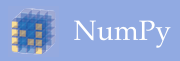
\includegraphics[width=100px]{../Notes/img/numpy.png}
  \end{center}
  \begin{itemize}
    \item $n$-dimensionale Arrays
    \item Funktionen, die auf denen arbeiten
    \item Operatoren wirken elementweise
    \item wird meist mit \texttt{np} abgekürzt
  \end{itemize}

  Konstanten:
  \begin{itemize}
    \item \texttt{pi}
    \item \texttt{e}
  \end{itemize}
\end{frame}

\begin{frame}{Arrays erstellen}
  \begin{itemize}
    \item \texttt{array}: konvertiert irgendwas (Liste, Tupel, …) zu einem Array
    \item \texttt{linspace(start, end, number)}: Array aus \texttt{number} Zahlen zwischen \texttt{start} und \texttt{end} in gleichem Abstand
    \item \texttt{arange(start, end, step)}: Array aus Zahlen zwischen \texttt{start} und \texttt{end} mit dem Abstand \texttt{step}
    \item \texttt{zeros(shape)}: Array aus Nullen der Größe \texttt{shape}
    \item \texttt{ones(shape)}: Array aus Einsen der Größe \texttt{shape}
  \end{itemize}
\end{frame}

\begin{frame}{Elementweise Funktionen}
  Beispiele:
  \begin{itemize}
    \item \texttt{sqrt}
    \item \texttt{exp}, \texttt{log}
    \item \texttt{sin}
    \item \texttt{deg2rad}, \texttt{rad2deg}
  \end{itemize}
\end{frame}

\begin{frame}{Reduzierende Funktionen}
  Beispiele:
  \begin{itemize}
    \item \texttt{sum}
    \item \texttt{mean}
    \item \texttt{max}, \texttt{min}
    \item \texttt{ediff1d}
  \end{itemize}
\end{frame}

\begin{frame}{It/Output}
  \begin{itemize}
    \item \texttt{loadtxt(file [, unpack=True])}: Lädt eine Datei in ein Array.
      \texttt{unpack=True} transponiert das Array
    \item \texttt{savetxt(file, array)}: Speichert ein Array in eine Datei
  \end{itemize}
\end{frame}

\subsubsection{SciPy}
\begin{frame}{SciPy}
  \begin{center}
    
\includegraphics{../Notes/img/scipy.pdf}
  \end{center}
\end{frame}

\begin{frame}{Nützliche Funktionen}
  \begin{itemize}
    \item \texttt{optimize.curve\_fit}: fittet nichtlineare Funktionen
    \item \texttt{stats.sem}: gibt den Fehler des Mittelwerts
    \item \texttt{constants.C2K}: konvertiert Celsius in Kelvin
    \item \texttt{constants.K2C}: konvertiert Kelvin in Celsius
  \end{itemize}
\end{frame}

\begin{frame}{Konstanten}
  \begin{itemize}
    \item \texttt{scipy.constants.physical\_constants}: enthält diverse physikalische Konstanten, ihre Fehler und Einheiten (aus CODATA)
  \end{itemize}
\end{frame}

\subsubsection{matplotlib}
\begin{frame}{matplotlib}
  \begin{center}
    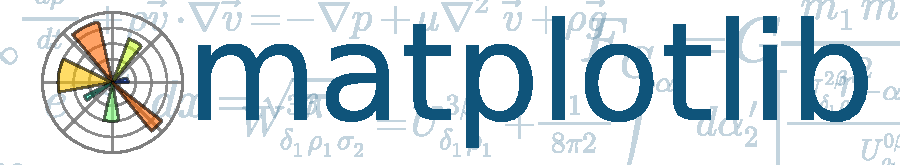
\includegraphics[width=\textwidth]{../Notes/img/matplotlib.pdf}
  \end{center}
  \begin{itemize}
    \item prozedurales Interface (in PyLab)
    \item objektorientiertes Interface (im Skript)
  \end{itemize}
\end{frame}
